% Options for packages loaded elsewhere
\PassOptionsToPackage{unicode}{hyperref}
\PassOptionsToPackage{hyphens}{url}
%
\documentclass[
]{article}
\usepackage{amsmath,amssymb}
\usepackage{lmodern}
\usepackage{iftex}
\ifPDFTeX
  \usepackage[T1]{fontenc}
  \usepackage[utf8]{inputenc}
  \usepackage{textcomp} % provide euro and other symbols
\else % if luatex or xetex
  \usepackage{unicode-math}
  \defaultfontfeatures{Scale=MatchLowercase}
  \defaultfontfeatures[\rmfamily]{Ligatures=TeX,Scale=1}
\fi
% Use upquote if available, for straight quotes in verbatim environments
\IfFileExists{upquote.sty}{\usepackage{upquote}}{}
\IfFileExists{microtype.sty}{% use microtype if available
  \usepackage[]{microtype}
  \UseMicrotypeSet[protrusion]{basicmath} % disable protrusion for tt fonts
}{}
\makeatletter
\@ifundefined{KOMAClassName}{% if non-KOMA class
  \IfFileExists{parskip.sty}{%
    \usepackage{parskip}
  }{% else
    \setlength{\parindent}{0pt}
    \setlength{\parskip}{6pt plus 2pt minus 1pt}}
}{% if KOMA class
  \KOMAoptions{parskip=half}}
\makeatother
\usepackage{xcolor}
\usepackage[margin=1in]{geometry}
\usepackage{color}
\usepackage{fancyvrb}
\newcommand{\VerbBar}{|}
\newcommand{\VERB}{\Verb[commandchars=\\\{\}]}
\DefineVerbatimEnvironment{Highlighting}{Verbatim}{commandchars=\\\{\}}
% Add ',fontsize=\small' for more characters per line
\usepackage{framed}
\definecolor{shadecolor}{RGB}{248,248,248}
\newenvironment{Shaded}{\begin{snugshade}}{\end{snugshade}}
\newcommand{\AlertTok}[1]{\textcolor[rgb]{0.94,0.16,0.16}{#1}}
\newcommand{\AnnotationTok}[1]{\textcolor[rgb]{0.56,0.35,0.01}{\textbf{\textit{#1}}}}
\newcommand{\AttributeTok}[1]{\textcolor[rgb]{0.77,0.63,0.00}{#1}}
\newcommand{\BaseNTok}[1]{\textcolor[rgb]{0.00,0.00,0.81}{#1}}
\newcommand{\BuiltInTok}[1]{#1}
\newcommand{\CharTok}[1]{\textcolor[rgb]{0.31,0.60,0.02}{#1}}
\newcommand{\CommentTok}[1]{\textcolor[rgb]{0.56,0.35,0.01}{\textit{#1}}}
\newcommand{\CommentVarTok}[1]{\textcolor[rgb]{0.56,0.35,0.01}{\textbf{\textit{#1}}}}
\newcommand{\ConstantTok}[1]{\textcolor[rgb]{0.00,0.00,0.00}{#1}}
\newcommand{\ControlFlowTok}[1]{\textcolor[rgb]{0.13,0.29,0.53}{\textbf{#1}}}
\newcommand{\DataTypeTok}[1]{\textcolor[rgb]{0.13,0.29,0.53}{#1}}
\newcommand{\DecValTok}[1]{\textcolor[rgb]{0.00,0.00,0.81}{#1}}
\newcommand{\DocumentationTok}[1]{\textcolor[rgb]{0.56,0.35,0.01}{\textbf{\textit{#1}}}}
\newcommand{\ErrorTok}[1]{\textcolor[rgb]{0.64,0.00,0.00}{\textbf{#1}}}
\newcommand{\ExtensionTok}[1]{#1}
\newcommand{\FloatTok}[1]{\textcolor[rgb]{0.00,0.00,0.81}{#1}}
\newcommand{\FunctionTok}[1]{\textcolor[rgb]{0.00,0.00,0.00}{#1}}
\newcommand{\ImportTok}[1]{#1}
\newcommand{\InformationTok}[1]{\textcolor[rgb]{0.56,0.35,0.01}{\textbf{\textit{#1}}}}
\newcommand{\KeywordTok}[1]{\textcolor[rgb]{0.13,0.29,0.53}{\textbf{#1}}}
\newcommand{\NormalTok}[1]{#1}
\newcommand{\OperatorTok}[1]{\textcolor[rgb]{0.81,0.36,0.00}{\textbf{#1}}}
\newcommand{\OtherTok}[1]{\textcolor[rgb]{0.56,0.35,0.01}{#1}}
\newcommand{\PreprocessorTok}[1]{\textcolor[rgb]{0.56,0.35,0.01}{\textit{#1}}}
\newcommand{\RegionMarkerTok}[1]{#1}
\newcommand{\SpecialCharTok}[1]{\textcolor[rgb]{0.00,0.00,0.00}{#1}}
\newcommand{\SpecialStringTok}[1]{\textcolor[rgb]{0.31,0.60,0.02}{#1}}
\newcommand{\StringTok}[1]{\textcolor[rgb]{0.31,0.60,0.02}{#1}}
\newcommand{\VariableTok}[1]{\textcolor[rgb]{0.00,0.00,0.00}{#1}}
\newcommand{\VerbatimStringTok}[1]{\textcolor[rgb]{0.31,0.60,0.02}{#1}}
\newcommand{\WarningTok}[1]{\textcolor[rgb]{0.56,0.35,0.01}{\textbf{\textit{#1}}}}
\usepackage{graphicx}
\makeatletter
\def\maxwidth{\ifdim\Gin@nat@width>\linewidth\linewidth\else\Gin@nat@width\fi}
\def\maxheight{\ifdim\Gin@nat@height>\textheight\textheight\else\Gin@nat@height\fi}
\makeatother
% Scale images if necessary, so that they will not overflow the page
% margins by default, and it is still possible to overwrite the defaults
% using explicit options in \includegraphics[width, height, ...]{}
\setkeys{Gin}{width=\maxwidth,height=\maxheight,keepaspectratio}
% Set default figure placement to htbp
\makeatletter
\def\fps@figure{htbp}
\makeatother
\setlength{\emergencystretch}{3em} % prevent overfull lines
\providecommand{\tightlist}{%
  \setlength{\itemsep}{0pt}\setlength{\parskip}{0pt}}
\setcounter{secnumdepth}{-\maxdimen} % remove section numbering
\ifLuaTeX
  \usepackage{selnolig}  % disable illegal ligatures
\fi
\IfFileExists{bookmark.sty}{\usepackage{bookmark}}{\usepackage{hyperref}}
\IfFileExists{xurl.sty}{\usepackage{xurl}}{} % add URL line breaks if available
\urlstyle{same} % disable monospaced font for URLs
\hypersetup{
  pdftitle={analyze the ToothGrowth data},
  pdfauthor={ismael},
  hidelinks,
  pdfcreator={LaTeX via pandoc}}

\title{analyze the ToothGrowth data}
\author{ismael}
\date{2022-09-21}

\begin{document}
\maketitle

\hypertarget{overview}{%
\subsection{Overview}\label{overview}}

we're going to analyze the ToothGrowth data in the R datasets package.
Load the ToothGrowth data and perform some basic exploratory data
analyses Provide a basic summary of the data. Use confidence intervals
and/or hypothesis tests to compare tooth growth by supp and dose. (Only
use the techniques from class, even if there's other approaches worth
considering) State your conclusions and the assumptions needed for your
conclusions.

\hypertarget{load-the-toothgrowth-data-and-perform-exploratory-data-analyses}{%
\subsection{Load the ToothGrowth data and perform exploratory data
analyses}\label{load-the-toothgrowth-data-and-perform-exploratory-data-analyses}}

\begin{verbatim}
## Warning: package 'ggplot2' was built under R version 4.2.1
\end{verbatim}

\begin{verbatim}
## 'data.frame':    60 obs. of  3 variables:
##  $ len : num  4.2 11.5 7.3 5.8 6.4 10 11.2 11.2 5.2 7 ...
##  $ supp: Factor w/ 2 levels "OJ","VC": 2 2 2 2 2 2 2 2 2 2 ...
##  $ dose: num  0.5 0.5 0.5 0.5 0.5 0.5 0.5 0.5 0.5 0.5 ...
\end{verbatim}

\begin{verbatim}
##    len supp dose
## 1  4.2   VC  0.5
## 2 11.5   VC  0.5
## 3  7.3   VC  0.5
## 4  5.8   VC  0.5
## 5  6.4   VC  0.5
## 6 10.0   VC  0.5
\end{verbatim}

\begin{verbatim}
##       len        supp         dose      
##  Min.   : 4.20   OJ:30   Min.   :0.500  
##  1st Qu.:13.07   VC:30   1st Qu.:0.500  
##  Median :19.25           Median :1.000  
##  Mean   :18.81           Mean   :1.167  
##  3rd Qu.:25.27           3rd Qu.:2.000  
##  Max.   :33.90           Max.   :2.000
\end{verbatim}

\begin{Shaded}
\begin{Highlighting}[]
\NormalTok{TG }\OtherTok{=}\NormalTok{ ToothGrowth}
\FunctionTok{levels}\NormalTok{(TG}\SpecialCharTok{$}\NormalTok{supp) }\OtherTok{\textless{}{-}} \FunctionTok{c}\NormalTok{(}\StringTok{"Orange Juice"}\NormalTok{, }\StringTok{"Ascorbic Acid"}\NormalTok{)}
\FunctionTok{ggplot}\NormalTok{(TG, }\FunctionTok{aes}\NormalTok{(}\AttributeTok{x=}\FunctionTok{factor}\NormalTok{(dose), }\AttributeTok{y=}\NormalTok{len)) }\SpecialCharTok{+} 
  \FunctionTok{facet\_grid}\NormalTok{(.}\SpecialCharTok{\textasciitilde{}}\NormalTok{supp) }\SpecialCharTok{+}
  \FunctionTok{geom\_boxplot}\NormalTok{(}\FunctionTok{aes}\NormalTok{(}\AttributeTok{fill =}\NormalTok{ supp), }\AttributeTok{show\_guide =} \ConstantTok{FALSE}\NormalTok{) }\SpecialCharTok{+}
  \FunctionTok{labs}\NormalTok{(}\AttributeTok{title=}\StringTok{"tooth length by dosage"}\NormalTok{, }
    \AttributeTok{x=}\StringTok{"Dose (mg/day)"}\NormalTok{,}
    \AttributeTok{y=}\StringTok{"Tooth Length"}\NormalTok{)}
\end{Highlighting}
\end{Shaded}

\begin{verbatim}
## Warning: `show_guide` has been deprecated. Please use `show.legend` instead.
\end{verbatim}

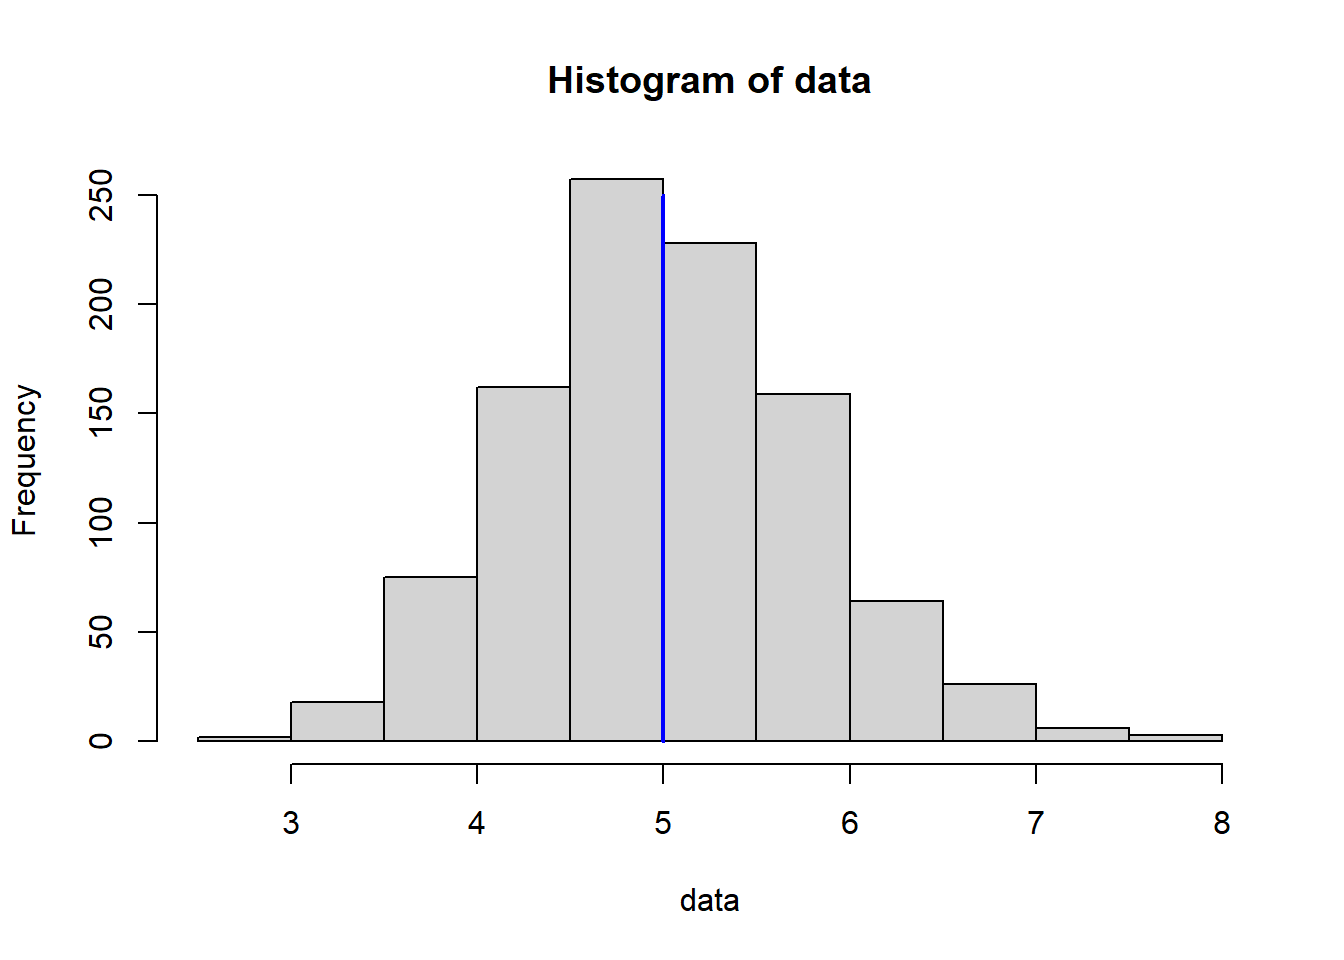
\includegraphics{Course-Project-Part-2_files/figure-latex/unnamed-chunk-2-1.pdf}

\hypertarget{basic-summary-of-the-data}{%
\subsection{Basic summary of the data}\label{basic-summary-of-the-data}}

looking at our plot, It seems that when Dosage of both types of
supplements increase, Tooth Length increase and also that Ascorbic acid
is less effective than Orange juice under 2.0 milligrams per day.

\hypertarget{use-confidence-intervals-hypothesis-tests-to-compare-tooth-growth-by-supplement-and-dose}{%
\subsection{Use confidence intervals \& hypothesis tests to compare
tooth growth by supplement and
dose}\label{use-confidence-intervals-hypothesis-tests-to-compare-tooth-growth-by-supplement-and-dose}}

\hypertarget{tooth-growth-by-supplement}{%
\paragraph{tooth growth by
supplement}\label{tooth-growth-by-supplement}}

\begin{Shaded}
\begin{Highlighting}[]
\FunctionTok{t.test}\NormalTok{(len }\SpecialCharTok{\textasciitilde{}}\NormalTok{ supp, ToothGrowth)}
\end{Highlighting}
\end{Shaded}

\begin{verbatim}
## 
##  Welch Two Sample t-test
## 
## data:  len by supp
## t = 1.9153, df = 55.309, p-value = 0.06063
## alternative hypothesis: true difference in means between group OJ and group VC is not equal to 0
## 95 percent confidence interval:
##  -0.1710156  7.5710156
## sample estimates:
## mean in group OJ mean in group VC 
##         20.66333         16.96333
\end{verbatim}

The p-value is 0.06 witch is greater than 0.05 and confidence interval
includes zero In conclusion, supplements types have no impact on Tooth
growth.

\hypertarget{tooth-growth-by-dose}{%
\paragraph{tooth growth by dose}\label{tooth-growth-by-dose}}

\begin{Shaded}
\begin{Highlighting}[]
\FunctionTok{t.test}\NormalTok{(len }\SpecialCharTok{\textasciitilde{}}\NormalTok{ dose, ToothGrowth[ToothGrowth}\SpecialCharTok{$}\NormalTok{dose }\SpecialCharTok{\%in\%} \FunctionTok{c}\NormalTok{(}\FloatTok{0.5}\NormalTok{, }\DecValTok{1}\NormalTok{), ])}
\end{Highlighting}
\end{Shaded}

\begin{verbatim}
## 
##  Welch Two Sample t-test
## 
## data:  len by dose
## t = -6.4766, df = 37.986, p-value = 1.268e-07
## alternative hypothesis: true difference in means between group 0.5 and group 1 is not equal to 0
## 95 percent confidence interval:
##  -11.983781  -6.276219
## sample estimates:
## mean in group 0.5   mean in group 1 
##            10.605            19.735
\end{verbatim}

\begin{Shaded}
\begin{Highlighting}[]
\FunctionTok{t.test}\NormalTok{(len }\SpecialCharTok{\textasciitilde{}}\NormalTok{ dose, ToothGrowth[ToothGrowth}\SpecialCharTok{$}\NormalTok{dose }\SpecialCharTok{\%in\%} \FunctionTok{c}\NormalTok{(}\DecValTok{1}\NormalTok{, }\DecValTok{2}\NormalTok{), ])}
\end{Highlighting}
\end{Shaded}

\begin{verbatim}
## 
##  Welch Two Sample t-test
## 
## data:  len by dose
## t = -4.9005, df = 37.101, p-value = 1.906e-05
## alternative hypothesis: true difference in means between group 1 and group 2 is not equal to 0
## 95 percent confidence interval:
##  -8.996481 -3.733519
## sample estimates:
## mean in group 1 mean in group 2 
##          19.735          26.100
\end{verbatim}

The p-value is near zero and confidence interval is less than zero. In
conclusion, the average of tooth length increases with dose so the null
hypothesis is rejected.

\hypertarget{conclusions-and-assumptions}{%
\paragraph{Conclusions and
Assumptions}\label{conclusions-and-assumptions}}

looking at the results of our tests, increase the dose also increase the
tooth growth, but supplement type has no effect on tooth growth.

\end{document}
